%\documentclass[]{article}
\documentclass[letterpaper, paper,11pt]{AAS}
\usepackage{amssymb}
\usepackage{amsmath}
\usepackage{graphicx}
\usepackage{amsthm}
\newtheorem{theorem}{Theorem}

% Title Page
\title{Entry Guidance for Propellant Optimal Powered Descent Ignition on Mars}


\PaperNumber{20-664}
\begin{document}
\author{Connor D. Noyes\thanks{Ph.D. Candidate, Department of Mechanical and Aerospace Engineering, University of California, Irvine, 92697} \ and Kenneth D. Mease\thanks{Professor Emeritus, Department of Mechanical and Aerospace Engineering, University of California, Irvine, 92697}}
\maketitle

\begin{abstract}
Powered descent plays an important role in current Mars entry, descent, and landing operations, and its importance will only grow as future missions begin to utilize supersonic retropropulsion to deliver heavier payloads to the surface with pinpoint accuracy. In current Mars entry trajectories, bank angle modulation provides range control prior to parachute deployment. Our approach represents a paradigm shift in which the entry guidance objective is to deliver the vehicle to propellant-optimal ignition conditions for a chosen powered descent guidance. The powered descent guidance is used to define a target set, and a mapping from that target set to the propellant required for pinpoint landing. The proposed entry guidance uses this target, which allows us to explicitly coordinate the entry guidance with powered descent guidance, and propellant savings can be realized relative to traditional entry guidance.  The approach is tested in a 1000 sample Monte Carlo simulation.
\end{abstract}

\section{Introduction}
Among the many considerable challenges involved in the Entry, Descent, and Landing (EDL) of a spacecraft on Mars, perhaps the greatest is the low density of the Martian atmosphere \cite{BraunMarsEDL, joel_dissertation}. At approximately one percent of the Earth's atmospheric density, current generation Mars entry vehicles are incapable of achieving sufficient deceleration to reach subsonic speeds before reaching the surface, necessitating the use of EDL technologies including supersonic parachutes and retropropulsion, both of which were utilized in safely landing MSL's Curiosity rover \cite{MSL_EDL}, and will also be utilized on the upcoming Mars 2020 mission \cite{M2020_EDL}. As the mass (or ballistic coefficient) of these vehicles grows, the problem is exacerbated until safe deployment conditions for current supersonic parachutes are not reachable at altitudes high enough to provide sufficient timeline margin for subsequent EDL events \cite{BraunMarsEDL}. In such missions, supersonic retropropulsion (SRP) may be relied upon to land larger, heavier vehicles relative to the current generation of landers without the use of a parachute, and as a result powered descent will play an even more significant role in the EDL process. In this paper, the emphasis is on the interplay between the entry phase and the powered phase, and thus only these two phases are considered.

%\textbf{It might be good to talk about the two phases here.}Figure~\ref{fig_phases} shows the two-phase EDL problem under consideration. 
The challenges during the entry phase from a guidance perspective include entry state dispersions due to delivery errors, atmospheric winds and density uncertainty, aerodynamic uncertainty, and imperfect onboard state estimation, each of which contribute to the size of the landing footprint. To date, MSL is the only Mars entry system to utilize hypersonic guidance to autonomously steer the spacecraft toward the target, which resulted in a landing footprint nearly an order of magnitude smaller than previous unguided ballistic entries \cite{BraunMarsEDL}. 
It is expected that a feature of SRP-based EDL is the requirement for pinpoint accuracy, defined as a sub-100 meter landing ellipse \cite{GNC_Pinpoint}. Assuming an entry guidance meets the basic requirement of delivering the vehicle to a state from which the powered guidance can achieve pinpoint landing, dispersed entry trajectories result in increased propellant requirements, rather than contribute to the landing ellipse. As a result, rather than judge an entry guidance algorithm by its landing ellipse, the propellant cost or propellant mass fraction (PMF) of the powered descent trajectory may now be considered a primary metric.

A fundamental difference of retropropulsion-based EDL from parachute-based EDL architectures, even those that utilize a vertical powered descent phase with potential for a divert maneuver beforehand, lies in the set of desirable states at the termination of the entry phase. In parachute-based EDL, the terminal entry state is constrained by safe parachute deployment conditions defined by upper and lower limits on Mach number and dynamic pressure. The constraints are often translated into constraints on altitude and velocity using a model of the Martian atmosphere. In summary, when a chute is involved, the target set for entry guidance is the parachute deployment box coupled with small downrange and crossrange errors, combined with a well-aligned heading, and no restriction on flight path angle. 

Traditionally, the primary objective of bank angle modulation during entry is range control with lateral control as a secondary objective, and guidance approaches could treat the two problems as decoupled. During the mission design phase, the downrange distance is chosen to be compatible with the parachute deployment conditions and other mission parameters such as the entry flight path angle. The target set in SRP-based EDL is in some sense much larger, but with more coupling between the state variables because, for a given powered descent guidance, the final entry state determines if pinpoint landing can be achieved, and if so, the propellant mass required. All six entry state variables contribute to the propellant cost; the optimal downrange distance and altitude at which to ignite depend on both the velocity magnitude and the flight path angle, while aligning the heading eliminates crosstrack flight during powered descent. 

% Altering the objective of entry guidance to shaping the trajectory for the benefit of the powered descent phase thus encourages a coupled approach. 
%For example, MSL utilized a range control phase and a heading alignment phase. Once the heading is aligned, the bank angle command will remain zero until the termination of the entry phase. Thus, unless heading alignment is initiated at the right time for zero bank angle to lead to the best termination condition, blah blah.

There exist many guidance solutions to the powered descent problem, often with a focus on propellant optimality. Classes of such algorithms include G-FOLD \cite{gfold,gfold_flighttests} and other convex optimization-based methods, polynomial-based approaches including the venerated Apollo lunar descent guidance \cite{apollo_lunar}, indirect optimal control methods \cite{PropellantOptimalAdaptiveTrigger}, and many others. 

Far less attention has been given to the role of entry guidance when followed directly by a powered descent phase, without an intermediate phase that makes use of a parachute or other decelerator. Reference~\cite{LuAdaptiveEDL} presents one approach to entry guidance in a chuteless EDL architecture. Reference~\cite{LuAdaptiveEDL} correctly identifies the potential for integrating the entry phase with the subsequent powered descent phase as an opportunity to reduce propellant consumption, and the vehicle bank angle is modulated to perform range control, utilizing a bank profile that is linear-in-energy with one free parameter. Lateral logic to determine bank reversals is applied separately after solving for the bank angle magnitude. Reference~\cite{EDL_AllProp} investigated an alternative EDL scheme in which aerodynamic control during entry is foregone in favor of hypersonic retropropulsion, essentially eliminating the entry phase. 

The proposed entry guidance for SRP-based EDL is designed to deliver the vehicle to a target set of states from which pinpoint landing can be achieved in the subsequent powered descent phase. Of the reachable states in the target set, entry guidance steers the vehicle to the one that will require the minimum propellant mass for pinpoint landing. For the simulation testing in this paper, the target set is computed by solving optimal control problems. 
%Details of this computation are presented later. This mapping is utilized in two distinct ways. At points along a given entry trajectory, the propellant cost can be computed in order to determine the best ignition condition for that trajectory. Additionally, the bank angle profile can be modified to intersect a portion of the feasible ignition set with sufficiently low propellant cost, using the mapping.  
%If the trajectory is poor, there may be not suitable ignition point, and the bank angle profile should be modified.
The possibility of computing the powered descent controllable set to be used as a target set for an entry guidance algorithm was suggested in Ref.~\cite{SRP_ControllableSets}, wherein a procedure based on convex optimization was designed to efficiently compute it is given.

MSL triggered its parachute deployment and descent sequence using a velocity trigger \cite{MSL_EDL}, while Mars 2020 will utilize a range trigger \cite{M2020_EDL} to dramatically decrease the size of the landing ellipse \cite{TriggerComparison2020}. A component of our approach is an onboard determination of when to trigger powered descent initiation.  In essence, the role of such a trigger is to ensure the minimum propellant ignition point is found along any entry trajectory that has at least one feasible ignition state. The theoretical developments behind one such trigger were introduced in Ref.~\cite{PropellantOptimalAdaptiveTrigger}, while Ref.~\cite{LuAdaptiveEDL} demonstrated its benefits over triggering at a fixed state variable, such as downrange, velocity, or energy.
One potential weakness of the trigger in Ref.~\cite{PropellantOptimalAdaptiveTrigger} is that it assumes a propellant optimal powered descent guidance. In theory, future Mars missions, especially those transporting humans, may very well consider a guidance algorithm with a different objective, such as prioritizing safety or even passenger comfort, as the bang-bang nature of propellant optimal powered descent solutions may not be suitable, despite the importance of limiting propellant consumption. 

Despite presenting an approach in which a prediction of the terminal entry state is available and being used to modulate the vehicle bank angle, in Ref.~\cite{LuAdaptiveEDL} only the current vehicle state is checked for triggering the powered descent initiation. Our approach to the triggering mechanism differs in that we utilize the predicted trajectory. This allows us to query the mapping from the powered descent guidance algorithm at points along the predicted trajectory to generate propellant consumption predictions.  The benefit of doing so is two-fold. Firstly, the propellant optimal ignition point along an entry trajectory can be determined for any subsequent powered descent guidance, even one that is itself not propellant optimal. Secondly, by making explicit use of these predictions in the entry guidance algorithm, the two phases become linked by more than just the onboard triggering strategy, and superior propellant performance can be achieved. 

%Additionally, as mentioned above, our proposed entry guidance approach utilizes the powered descent guidance to be employed in the subsequent phase, in order to generate predicted propellant costs along a predicted trajectory. In this approach, the bank angle is actively modulated to reduce predicted propellant consumption rather than achieve a range objective, thereby allowing the entry guidance algorithm to suitably shape the trajectory in preparation for powered descent. It is this coordinated effort that allows the proposed entry guidance to produce superior results over traditional entry guidance methods. 

%We note that Reference Fully-Propulsive Mars Atmos Strategies for High-Mass Payload Missions looked at chuteless architectures but did not utilize lifting for control, and instead employed HYPERsonic retropulsion.
\section{Entry Guidance Problem}
The problem under investigation considers a two-phase EDL sequence consisting of an entry phase and a powered descent phase. The dispersions in vehicle state arising from the approach phase are modeled as delivery errors at the beginning of the EDL sequence. In the entry phase, the vehicle is guided via bank angle modulation and the vehicle state is described in spherical coordinates. In the descent phase, the vehicle is guided via supersonic retropropulsion with the equations of motion given in Cartesian coordinates.  The reason for the choice of two different coordinate systems is to be consistent with the literature on each respective topic.

\begin{figure}[h!]
	\centering
	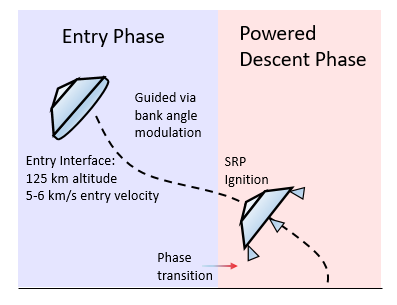
\includegraphics[width=0.5\textwidth]{EDLPhaseDiagram} 
	\caption{Schematic of the EDL phases}
	\label{fig_phases}
\end{figure}

The planet-relative equations of motion for a vehicle, modeled as a point mass, in unpowered flight through an atmosphere, in spherical coordinates, are
\begin{align}
\dot{R} &= V\sin\gamma \label{eq_entry_start}\\
\dot{\theta} &= \frac{V}{R}\frac{\cos\gamma\cos\psi}{\cos\phi}\\
\dot{\phi} &= \frac{V}{R}\cos\gamma\sin\psi \\
\dot{V} &= -D - G\sin\gamma \\
\dot{\gamma} &= \frac{L}{V}\cos\sigma + (\frac{V}{R}-\frac{G}{V})\cos\gamma + C_{\gamma}\\
\dot{\psi} &= -\frac{L}{V}\frac{\sin\sigma}{\cos\gamma} - \frac{V}{R}\cos^2\gamma\cos\psi\tan\phi + C_{\psi}\label{eq_entry_end}
\end{align}
where $R$ is magnitude of the vehicle's radial distance from the center of the planet, $\theta$ and $\phi$ are the longitude and latitude of the vehicle, $V$ is the magnitude of the vehicle's velocity vector,  $G=\mu/R^2$ is the magnitude of the gravitational acceleration, $\gamma$ is the flight path angle, $\psi$ defines the vehicle heading, measured counterclockwise from East, and $\sigma$ is the bank angle of the vehicle. The aerodynamic accelerations are computed 
\begin{align}
D &= \frac{1}{2}\rho V^2\frac{S}{m}C_D = \frac{q}{\beta} \\
L &= \frac{1}{2}\rho V^2\frac{S}{m}C_L = \frac{q}{\beta}\frac{C_L}{C_D} \\
\end{align}
where $ \rho $ is the atmospheric density, $S$ is the aerodynamic surface area, $q=\frac{1}{2}\rho V^2$ is the dynamic pressure, and $\beta = \frac{m}{SC_D}$ is the ballistic coefficient.
The Coriolis terms $C_{\gamma},\,C_{\psi}$ are equal to
\begin{align}
C_{\gamma} &= 2\omega\cos\psi\cos\phi \\
C_{\psi} &= 2\omega(\tan\gamma\sin\psi\cos\phi-\sin\phi)
\end{align}
where $\omega$ is the rotation rate of Mars. Equations~\ref{eq_entry_start}-\ref{eq_entry_end} will be compactly referred to as $\dot{\mathbf{x}} = f(\mathbf{x},\sigma)$ and their solution at time $t$ from a state $\mathbf{x_0}$ evolving under a bank angle profile $\sigma[0,t]$ is given by the transition map $\mathbf{x}(t) = \varphi(t;\, \mathbf{x_0},\,\sigma[0,\,t])$.

%By solving the powered descent problem on the ground over a set of possible ignition states, an entry target set may be defined that allows us to reduce the two-phase problem to a problem with only an entry phase. In this new problem, the propellant required to land is only a function of the terminal entry state, because the powered descent thrust vector profile and time of flight are no longer optimization variables. Instead, the entire powered descent trajectory is now a function of the terminal entry state.  Hence, 
The entry guidance problem is to determine the entry phase duration and a bank angle profile that will deliver the vehicle from the entry interface to the propellant-optimal point in the target set, i.e., the set from which pinpoint landing can achieved. A formal definition of the target set is given in the subsequent section.
%\begin{align}
%\min \mathrm{prop}(\mathbf{x}(t_{pd})) \label{eq_entry_ocp}\\
%&\mathbf{x}(t_0) = \mathbf{x_0} \\
%&\mathbf{x}(t_{pd}) \in \mathcal{F}_M \\
%&\dot{\mathbf{x}} = f(\mathbf{x},\sigma)
%\end{align}

\subsection{Entry Guidance Target Set}
The entry guidance target set is defined by the powered descent algorithm to be used during the descent phase, and the available propellant onboard the vehicle. The equations of motion for a point mass vehicle in powered flight in a surface fixed frame, neglecting aerodynamic forces and Coriolis effects, are
\begin{align}
&\dot{\mathbf{r}} = \mathbf{v} \label{eq_eom_srp} \\
&\dot{\mathbf{v}} = \frac{\mathbf{T}}{m} + \mathbf{g}(\mathbf{r}) \\
&\dot{m} = -\frac{||\mathbf{T}||}{I_{sp}G_0} \label{eq_eom_srp_end}
\end{align}
where $\mathbf{r}\in\mathbb{R}^3$ is the position vector of the vehicle, $\mathbf{v}\in\mathbb{R}^3$ is the velocity vector of the vehicle, $m$ is its mass, $\mathbf{T}\in\mathbb{R}^3$ is the thrust vector of the vehicle, $\mathbf{g}\in\mathbb{R}^3$ is the gravitational acceleration vector, $I_{sp}$ is the specific impulse of the rocket engine, assumed to be constant, and $G_0$ is the gravitational acceleration magnitude at the surface of the Earth. The full powered descent state vector in $\mathbb{R}^7$ comprises the position, velocity, and mass. 

%The powered descent problem considered herein is to determine the optimal thrust magnitude and direction, as well the optimal time of flight, that solve the pinpoint landing boundary value problem comprising the equations of motion with prescribed initial and final conditions, while subject to constraints on the available thrust. 
Any powered descent algorithm capable of meeting the pinpoint landing requirement may be considered. To eschew the choice of a specific algorithm in this paper, the powered descent problem is posed as the optimal control problem
\begin{align}
\max \;m(t_f) \label{eq_srp_ocp}\\
&\mathbf{r}(t_0) = \mathbf{r_0} \\
&\mathbf{v}(t_0) = \mathbf{v_0} \\
&m(t_0) = m_0\\
&\mathbf{r}(t_f) = [0,\, 0,\, z_{\mathrm{target}}] \\
&\mathbf{v}(t_f) = [0,\, 0,\, \dot{z}_{\mathrm{target}}] \\
0 <\,\, &T_{\min} \le ||\mathbf{T}(t)|| \le T_{\max}
\end{align}
%together with the dynamics Eq.~\ref{eq_eom_srp}-\ref{eq_eom_srp_end},
where the final time $t_f$ is free, $T_{\min}$ and $ T_{\max} $ are constant bounds on the available thrust, and $z_{\mathrm{target}}$ and $\dot{z}_{\mathrm{target}}$ are the desired altitude and vertical velocity at the end of the descent phase. For a fixed initial mass, maximizing the final mass is equivalent to minimizing the propellant use. Formulated as such, the optimal control problem can be viewed as a function $\mathrm{OCP}(\cdot)$ that maps an initial condition, i.e., ignition state, to a propellant cost. 
The set of initial states for which the optimal control problem has a feasible solution includes regions that are not of interest. Examples include states with initial altitudes very low to the ground, initial velocities much higher than those reachable by the entry vehicle before impacting the surface, and initial distances very far from the target, or having already overshot the target. Denoting $\mathbf{r} = [x,y,z]^T$, the set of feasible solutions is restricted to a region of interest by defining a set of constraints
\begin{equation}
c_i(\mathbf{x})\le 0\:\; \mathrm{for}\,\;i=\{1,2,3,4\}\\
\end{equation} where 
\begin{align}
\mathbf{c}(\mathbf{x}) = \left[ \begin{array}{lc}
        x^2 + y^2 - d^2_{\max}\\
        d^2_{\min} - x^2 - y^2\\
        z_{\mathrm{target}} + z_{\min} - z \\
        ||\textbf{v}|| - v_{\max}
        \end{array} \right]\label{eq_constraints} 
\end{align} 
%to be applied $c_i(\mathbf{x}) \le0\;\mathrm{for}\,i=1,...,4$, and where 
and $[d_{\min},\,d_{\max}]$ are the minimum and maximum distance to the target, $z_{\min}$ is the minimum altitude, and $v_{\max}$ is the upper bound on velocity. 
%Let the controllable set, $\mathcal{C}$, be defined as the set of initial states for which there exists a thrust control function that leads the vehicle to the specified final state. We assume that $\mathcal{C}$, and the set of initial states for which the optimal control problem has a solution, are the same. 
The set of all initial state vectors for which the solution to the optimal control problem is feasible and the propellant required by the solution is less than some prescribed maximum $ M $, and satisfying these constraints is 
\begin{align}
\mathcal{F}_{M} = \left\{\mathbf{x}\,|\, \max_{i={1,...,4}}c_i(\mathbf{x})\le 0\,\,\mathrm{and}\,\,\mathrm{OCP}(\mathbf{x}) \le M \right\},
\end{align}
and is the set targeted by the entry guidance algorithm. Although the set is used an entry guidance target, it is defined in terms powered descent state variables. As the initial T/W ratio of the vehicle increases, $\mathcal{F}_{M}$ contracts. This is because, for a fixed $I_{sp}$ and $T_{\min}$, increasing thrust will increase the mass flow rate and decrease the maximum time of powered flight, which naturally decreases the distance from the target the vehicle can fly. The effect is that higher T/W places more stringent requirements on the entry guidance target set unless additional propellant is added, or the value of $I_{sp}$ or $T_{\min}$ changes.

Given an entry state and target position, the corresponding descent state is determined by assuming the current heading $\psi$ defines the downrange direction. The downrange and crossrange distances to the target are computed via spherical trigonometry \cite{joel_dissertation}
\begin{align}
d &= \cos^{-1}\left(\sin\phi\sin\phi_{\mathrm{target}} +\cos\phi\cos\phi_{\mathrm{target}}\cos(\theta_{\mathrm{target}}-\theta)        \right) \\
\Psi &= \pi/2 - \mathrm{sign}(\theta_{\mathrm{target}}-\theta) \cos^{-1}\left(\frac{\sin\phi_{\mathrm{target}}-\sin\phi\cos d}{\cos\phi\sin d}  \right) \\
c &= \sin^{-1}\left(\sin d\,\sin(\psi-\Psi))\right)
\end{align}
\begin{align}
DR &= R_p\cos^{-1}\left(\frac{\cos d}{\cos c}\right)\\
CR &= R_pc
\end{align}
where $R_p$ is the planet radius. 
%The altitude above the target is computed by subtracting the target altitude $z_{\mathrm{target}}$ from the current altitude $h = R-R_p$ and 
The full powered descent state vector in terms of the entry state variables is $[DR,\, |CR|,\, R-R_P,\, -V\cos\gamma,\, 0,\, V\sin\gamma,\, m_0]^T$. Because the downrange direction is defined by the current heading angle, the crossrange velocity is always zero. Under the assumed dynamics and zero crossrange velocity, the sign of the crossrange to the target does not affect the propellant cost, and its absolute value is used.

By using a downrange-crossrange coordinate system based on the current heading, an infinite number of entry states map to the same SRP state as a result of this surjective transformation. Intuitively, this reflects the rotational symmetry of the problem around the $z$-axis, stemming from the fact that states $ x $ and $ y $ have identical dynamics. For the powered descent problem as posed, any initial state $[ x,\, y,\, z,\, \dot{x},\, \dot{y},\, \dot{z},\, m]$ such that $(z, \dot{z}, m)$ are fixed and 
\begin{align}
x^2 &+ y^2 = p^2 \\
\dot{x}^2 &+ \dot{y}^2 = v^2 \\
\psi &= \tan^{-1}(y/x) \\
\dot{x} &= -v\cos\psi \\
\dot{y} &= -v\sin\psi \\
\end{align}
lies along an iso-propellant contour defined by the horizontal distance and velocity magnitudes, $p$ and $v$. An alternative mapping from entry states to powered descent states is to convert the entry state and target to Cartesian coordinates and subtract them. Although this is a feasible option, it is not preferable because it would result that every entry state maps to a unique SRP state. This is undesirable because it requires a larger table of solutions encompassing all the possible Cartesian states.

\section{Proposed Entry Guidance}

%Components of entry guidance: 
%Bank angle parametrization
%SRP guidance -> N-D table of propellant costs -> Required to determine both hand off state and params to get there 
%Onboard determination of ``handoff" i.e. transition from Entry phase to SRP phase 

%TODO: Minimum propellant set may be more appropriate - don't know that the set is a single point
The objective is to deliver the vehicle to the minimum propellant ignition point in the feasible subset $\mathcal{F}_M$ that is reachable under the chosen bank angle parametrization from the current state. This is in contrast to prescribing ad hoc rules for the terminal entry set to reduce propellant consumption, such as minimizing velocity at a certain downrange distance to the target. 
%Seeking the optimal point requires that the terminal entry state be free of such constraints, i.e., it cannot be required to lie on a manifold defined by a fixed velocity or distance from the target. 
This objective is accomplished by the guidance algorithm using a nested computational structure. At the inner level, the propellant map is used to determine the optimal ignition point along each predicted trajectory. At the outer level, the bank angle profile is optimized to find the optimal ignition state that is reachable from the current vehicle state. To mitigate the complexity of determining the bank angle function during flight, a parametrization is chosen on the ground, and its parameters are repeatedly optimized during flight. Thus, the three key components of the approach are the powered descent propellant map, the bank angle parametrization, and the onboard determination of the vehicle state at which the entry phase ends and powered descent begins.  

\begin{figure}[h!]
	\centering
	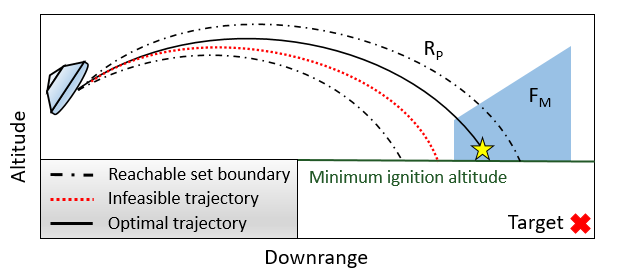
\includegraphics[width=0.8\textwidth]{Optimization} 
	\caption{The guidance algorithm seeks both the propellant-optimal ignition point (indicated by a star on the plot) and the trajectory whose optimal ignition point is best (indicated by the solid black line). The red, dotted trajectory is valid entry trajectory within the reachable set, but is infeasible because it does not intersect the powered descent feasible subset $\mathcal{F}_M$.}
	\label{fig_optimization}
\end{figure}

%At the core of the proposed entry phase guidance approach is an extension of the trajectory prediction to include the following powered descent phase. This allows one to alter the entry guidance objective from range control to propellant minimization. After applying several constraints to filter down the set of potential ignition states, the powered descent guidance is used to generate predictions of the propellant required from different states. The lowest among them is selected as the planned handoff condition from entry to powered descent. Further details on these constraints are given later.

%Notice that although propellant minimization is the entry guidance objective, any powered descent guidance algorithm with pinpoint landing capability may be used in the powered descent phase so long as an estimate of the propellant required is given by the algorithm, and this estimate is continuous with respect to the initial state. Thus, although in the examples of this work we have coordinated the powered descent phase to also be propellant-optimal in nature by solving the associated OCP, there exist many alternatives such as energy-optimal guidance or non-optimization based approaches such as polynomial guidance. 

%We further assume that the chosen powered descent method incorporates any necessary problem constraints, because the entry guidance algorithm does not make use of the predicted powered descent trajectory, nor does it check for satisfaction of constraints, but instead utilizes only the propellant cost associated with the powered descent trajectory. 
\subsection{Bank Angle Parametrization}
The entry phase guidance problem is intended to be solved onboard and so motivates a low-order parametrization of the bank angle profile. Parametrizing the bank angle function converts the optimal control problem into a more tractable nonlinear optimization problem. The choice of parametrization has important implications on the entry reachable set. The entry phase reachable set from an initial state $ \mathbf{x}_0$ is a tube of trajectories satisfying the equations of motion under admissible control functions 
\begin{equation*}
\mathcal{R}(\mathbf{x}_0)=\left\{\mathbf{x} \,| \,\exists\, t_f \;\mathrm{and}\; \sigma[0, t_f] \,\mathrm{with}\, \mathbf{x} = \varphi(t_f;\mathbf{x}_0,\, \sigma[0, t_f])  \right\}
\end{equation*}
and the portion of the reachable set that is of interest is its intersection with the powered descent feasible subset, i.e., $\mathcal{R} \cap \mathcal{F}_M$. Conceptually, by parametrizing the bank angle function in a particular way, we restrict the possible bank angle functions that can be generated, and as result will reduce the size of the reachable set. Let $R_P$ be the reachable set corresponding to a parametrization $ P $.
%The P-parametrized bank angle profile is a function of a finite set of parameters $P = \left\{p_1, p_2, ...,p_N \right\}$ and an associated function $h(\cdot)$ that defines the bank angle for each state, $\sigma(t) = h(P(x(t)))$.
%The dependence is to indicate closed loop nature, i.e. the values that P takes on change with the state unless flying perfectly along the optimal trajectory already 
%The P-parametrized reachable set is 
%\begin{equation*}
%\mathcal{R}(\mathbf{x}_0)=\left\{\mathbf{x} \,| \,\exists\, t_f \;\mathrm{and}\; \sigma(t)\,\forall\, t\in\,[0,t_f] \,\mathrm{with}\, \mathbf{x} = \varphi(\mathbf{x}_0; \sigma(t))  \right\}
%\end{equation*}
%$R_P(\mathbf{x}_0) =\left\{\mathbf{x}_f \,| \,\exists\, t_f \land\, P(\mathbf{x}) \,\mathrm{such\, that}\, \mathbf{x}_f = \varphi(t_f;\,\mathbf{x}_0,\, P(x(t))))  \right\} $. 
The relative size of $\mathcal{R}_P \subset \mathcal{R}$ is not the only consideration in choosing a parametrization. 
It is also desirable that $\mathcal{R}_P$ retains the propellant optimal point (or set) and neighboring region. 
%More formally, in addition to considering the effects of a parametrization on some measure of $\mathcal{R}_P\cap \mathcal{R}$, one may also consider the optimality gap, 
As a result, one might like to compare the propellant cost associated with a parametrization with the optimal solution over all parametrizations, i.e., compute
\begin{align}
\delta m = \left( \min_{x\in (\mathcal{R}\cap \mathcal{F}_M)} \mathrm{OCP}(x)\; - \min_{x\in (\mathcal{R}_P\cap \mathcal{F}_M)} \mathrm{OCP}(x) \right) \; \ge 0
\end{align}
in order to assess its quality, but this may be difficult to do. Instead, the minimum propellant costs of any two parametrizations can be compared against one another directly.  Let $\lambda$ be a measure of the volume of a state space set. Let $ P_A $ and  $ P_B $ be two different parametrizations, such that $\lambda(\mathcal{R}_{P_A}) < \lambda(\mathcal{R}_{P_B})$, and $\lambda(\mathcal{R}_{P_A}\cap \mathcal{R}) < \lambda(\mathcal{R}_{P_B}\cap \mathcal{R})$.
%but $\lambda(\mathcal{R}_{P_A}\cap \mathcal{F}_M) > \lambda(\mathcal{R}_{P_B}\cap \mathcal{F}_M)$.
Figure~\ref{fig_sets} depicts the relationship between the sets $\mathcal{F}_M,\,\mathcal{R},\,\mathcal{R}_{P_A},\,\mathrm{and}\,\mathcal{R}_{P_B}$ as well as a possible situation to demonstrate the possibility that $ \mathcal{R}_{P_A} $ is smaller than $\mathcal{R}_{P_B}$, and can reach less of $R$, yet has a smaller optimality gap than parametrization $ P_B $. 
\begin{figure}[h!]
	\centering
	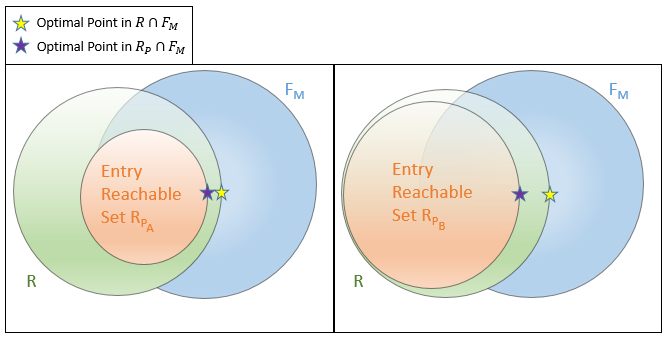
\includegraphics[width=0.9\textwidth]{SetDefinitions} 
	\caption{Consider two different parametrizations of the control, $ P_A $ and $ P_B $. While $ P_B $ allows the vehicle to reach more of the reachable set $\mathcal{R} $ than  $P_A$, much of $ R_{P_B}$ does not intersect $\mathcal{F}_M$. Additionally, the propellant optimal point in $ R_{P_A}$ is better than the optimal point in $ R_{P_B}$, indicated by the smaller distance between the optima, which are depicted with stars.  Note that these sets, depicted notionally as convex 2-D shapes, are actually 6-D and no claim is made about their convexity.}
	\label{fig_sets}
\end{figure}
%TODO: Better describe the stars? 
%Despite $ R_{P_B} $ being a larger set encompassing more of the true reachable set $R$, the intersection $R_{P_A}\cap \mathcal{F}_M$ is ``larger" than $R_{P_B}\cap \mathcal{F}_M$ and more importantly $ R_{P_A} $ encompasses a key subset of $ R $ – the region near the optimum. The difference between the two different optima is the sub-optimality gap imposed by the chosen parametrization.

The commanded bank angle profile considered here is a constant bank angle magnitude $\sigma_c$ with one bank reversal at a velocity $v_r$ and the current velocity $V$ is used as the independent variable in place of time,
\begin{equation}
\sigma(V; \sigma_c, \,v_r) = \left\{
\begin{array}{ll}
\sigma_c & V\geq v_r \\
-\sigma_c & V < v_r
\end{array} 
\right. .
\end{equation}
These commands are fed to a rate limiter to approximate the nature of a reaction control system tracking the commands. Because the profile includes a reversal, it offers a means to control lateral motion. 

The parametrization remains the same after the reversal, but the guidance continues to update the parameter values. By setting the lower bound on $v_r$ to be less than the ignition velocity during optimization, or greater than the current velocity, there exists the possibility to have one or no reversal planned at each update. This allows for as many reversals as there are optimization updates, but in simulations there will only be one or two reversals unless significant perturbations to the vehicle's planned heading occur after the first reversal. If an additional reversal is desired to eliminate large crossrange excursions, the parametrization is easily amended to accommodate one. A second reversal can be placed at a fixed velocity, and, exactly as the algorithm is currently applied, the first reversal timing is optimized until the reversal has been completed. Then, the second reversal is treated as the new optimization variable in addition to the bank angle magnitude. Such a ``one-at-a-time" strategy was put forth in Ref.~\cite{GuangfeiReplanning}. The result is, instead of one reversal with occasionally a second, all trajectories will feature two reversals with potential for a third. 

For comparison, we also consider a second parametrization of the form 
\begin{equation}
\sigma(V; \,v_1, \,v_2) = \left\{
\begin{array}{ll}
\;\;90^{\circ} & V\geq v_1 \\
-90^{\circ} & v_2 < V < v_1 \\
\;\;0^{\circ} & V \le v_2
\end{array} 
\right.
\end{equation}
where the two parameters $v_1,\, v_2$ such that $v_1 > v_2$ dictate the timing of the bank reversals, and the bank angle magnitudes are fixed.

\begin{figure}[h!]
		\centering
		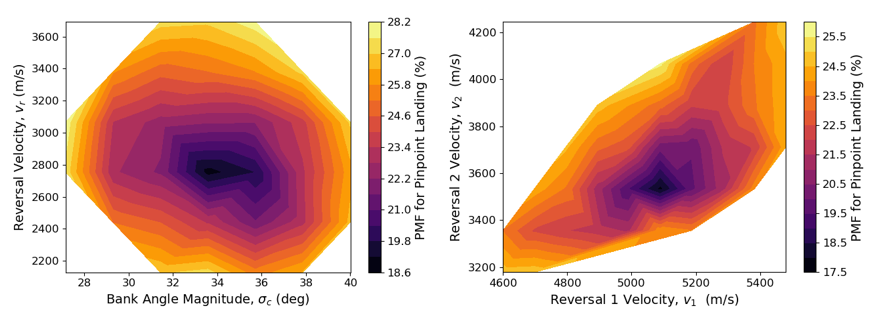
\includegraphics[width=1\textwidth]{ObjectiveContours} 
		\caption{Example contours of the propellant cost of pinpoint landing using two different parametrizations: a constant bank angle with one reversal, and a profile with two reversal velocities. Not only does the choice affect the propellant contours, but the reachable set is quite different as well. The downrange targeted in the constant profile is 700 km and is not reachable by the second parametrization, which instead targets 625 km. }
		\label{fig_objective_contour}
\end{figure}
%The entry guidance requires that the chosen powered descent guidance approach admits continuous propellant requirements for continuous ignition states to a fixed target. Atmospheric entry dynamics are smooth for smooth bank angle inputs and we thus expect that even when optimizing the ignition condition along a trajectory rather than use a fixed state variable such as velocity or energy, the objective function should be well-behaved and amenable to optimization. 
One key question when optimizing the parameters of the bank angle profile is whether there exist several isolated minima, or only a single global minimizer. 
Evaluating the objective function for a grid of the parameters defining the bank profile in each parametrization yields Figure~\ref{fig_objective_contour}, and indicates the objective function is likely convex, with steep gradients away from the optimum. From this, and repeated optimizations at various possible points, there is always a clear optimum.  The right plot of Figure~\ref{fig_objective_contour} shows that the two reversal parameters are significantly more coupled than the constant bank magnitude parametrization. This makes sense, as each reversal has a strong impact on the final heading, while in the constant bank parametrization, the bank magnitude has a much weaker affect on the heading than the reversal velocity. Clearly the choice of parametrization affects not only the shape of these contours, but also the minimum PMF achievable, as the second parametrization has a superior optimum. Note, however, that due to the difference in reachable set between the two parametrizations, the optimal downrange distance from the entry interface is different. For simplicity, the constant parametrization is adopted for the results in this paper. A more detailed analysis of the choice of parametrization is left for future work.

The shape of these objective functions indicates that gradient-based methods should be effective in determining the optimal profile parameters, however, determining the gradient of the objective function with respect to the switching velocity is generally difficult. As a result, derivative-free methods are preferred for this application. Powell's conjugate direction method \cite{PowellsMethod} is used in all of the examples herein. It is effective because for the chosen parametrization, the contours are nearly independent, so 1-D searches over each bounded parameter can very quickly locate the optimum. 

\subsection{Powered Descent Propellant Mapping}
By repeatedly solving the powered descent optimal control problem, Eq.~\ref{eq_srp_ocp}, for different ignition states, a pointwise approximation of a subset of the pinpoint landing feasible set $\mathcal{F}_M$ is computed via sampling. The full descent state vector is 7-D, but with two degenerate dimensions: the crossrange velocity, which is always zero by definition, and the initial mass, which is assumed to be fixed. A consequence of the dimensionality of the state space is a requirement to compute a large number of solutions -  16,807 solutions are required to span each of the remaining 5 dimensions with only 7 points. From sampled solutions we construct an approximation of the propellant costs for states in $\mathcal{F}_M$. Sampling is applicable irrespective of the powered descent algorithm to be used; for the problem of constrained propellant-optimal solutions, there exist significantly more efficient methods of computing the set $\mathcal{F}_M$ and the associated propellant cost, such as the convex optimization-based approach detailed in Ref.~\cite{SRP_ControllableSets}.

This mapping may be stored and interpolated in a variety of ways. Neural networks and other machine learning approaches were considered for their universal function approximation property. However, upon examination of the shape of the 5-D space together with numerical validation using additional OCP sample solutions, piecewise-linear 5-D interpolation was chosen to approximate the propellant mapping.
%The set of initial states over which to solve the OCP is computed by Latin Hypercube Sampling. After applying the constraints Eq~\ref{eq_constraints}, the OCP is solved for the remaining states. The model is constructed 
%TODO: Note (as Mease mentioned) that because the table is defined in SRP coordinates, it implicitly exploits the rotational symmetry as well 
%TODO: Iterative scheme
%TODO: Note the approximation is enabling, allowing MANY srp problems to be "solved" onboard
%, allowing the use of 5-D interpolation rather than 6-D. The absolute value of the crossrange distance is used because this gives a denser table of tabulated solutions by exploiting symmetry resulting from the zero crossrange velocity. 

\subsection{Trajectory Prediction and Powered Descent Ignition}
Once the bank angle parametrization is specified, the estimated entry state is integrated numerically to generate a prediction of the remaining unpowered entry trajectory. The components of the constraint vector Eq.~\ref{eq_constraints} used in the definition of $\mathcal{F}_M$ are then applied to the predicted trajectory to determine the interval that should be checked for the propellant-optimal transition to powered descent. These constraints greatly reduce the number of calls to the descent guidance propellant mapping required to find the optimum. As a reminder, these constraints include an upper bound on velocity corresponding to the maximum achievable deceleration with the available propellant, a minimum ignition altitude required for safe powered descent and subsequent EDL operations, and a maximum distance to the target, again related to the available propellant. Figure~\ref{fig_ignition} depicts this process including a portion of the trajectory already flown, the entry flight prediction, constraints, pinpoint landing target, and predicted optimal ignition point. 

Once the constraints have been applied, 1-D optimization is applied to the remaining trajectory interval, indicated by the dash black line, by viewing the fixed trajectory as a function of some independent variable. Our implementation uses velocity as the independent variable over which to search, but time or distance are also possibilities. 1-D optimization is used to very quickly locate the optimum, rather than determine the solution by brute force by checking all of the remaining points. Once the solution is determined, the commanded bank angle sign and magnitude are computed as a function of the vehicle estimated velocity, and are then sent to the control system.
%The numerical integration of the entry state is carried out using downrange distance to the target as the independent variable. Using range to go as the independent variable allows the terminal integration condition to be zero, independent of the problem specifics, with very little wasted integration time since the optimal ignition state is generally close to the target. 
%This has several advantages over common alternatives. First, although energy or velocity could be used, a sufficiently low choice of the terminal value must be made, but any time spent integrating below the reachable set of the vehicle is wasted, and the choice is problem/vehicle specific. Altitude would also be a natural choice since the minimum ignition altitude would serve as the terminal integration condition, but like energy and velocity this is problem-dependent, and additionally altitude is not a strictly monotonic variable in the case of lofting trajectories.
\begin{figure}[h!]
	\centering
	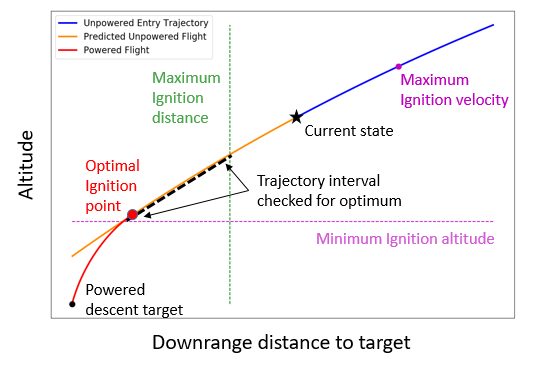
\includegraphics[width=0.7\textwidth]{H_Vs_S} 
	\caption{Only the interval of the predicted entry trajectory satisfying constraints on velocity, altitude, and distance to the target are searched for the propellant-optimal ignition state.}
	\label{fig_ignition}
\end{figure}

%\begin{figure}[h!]
%		\centering
%		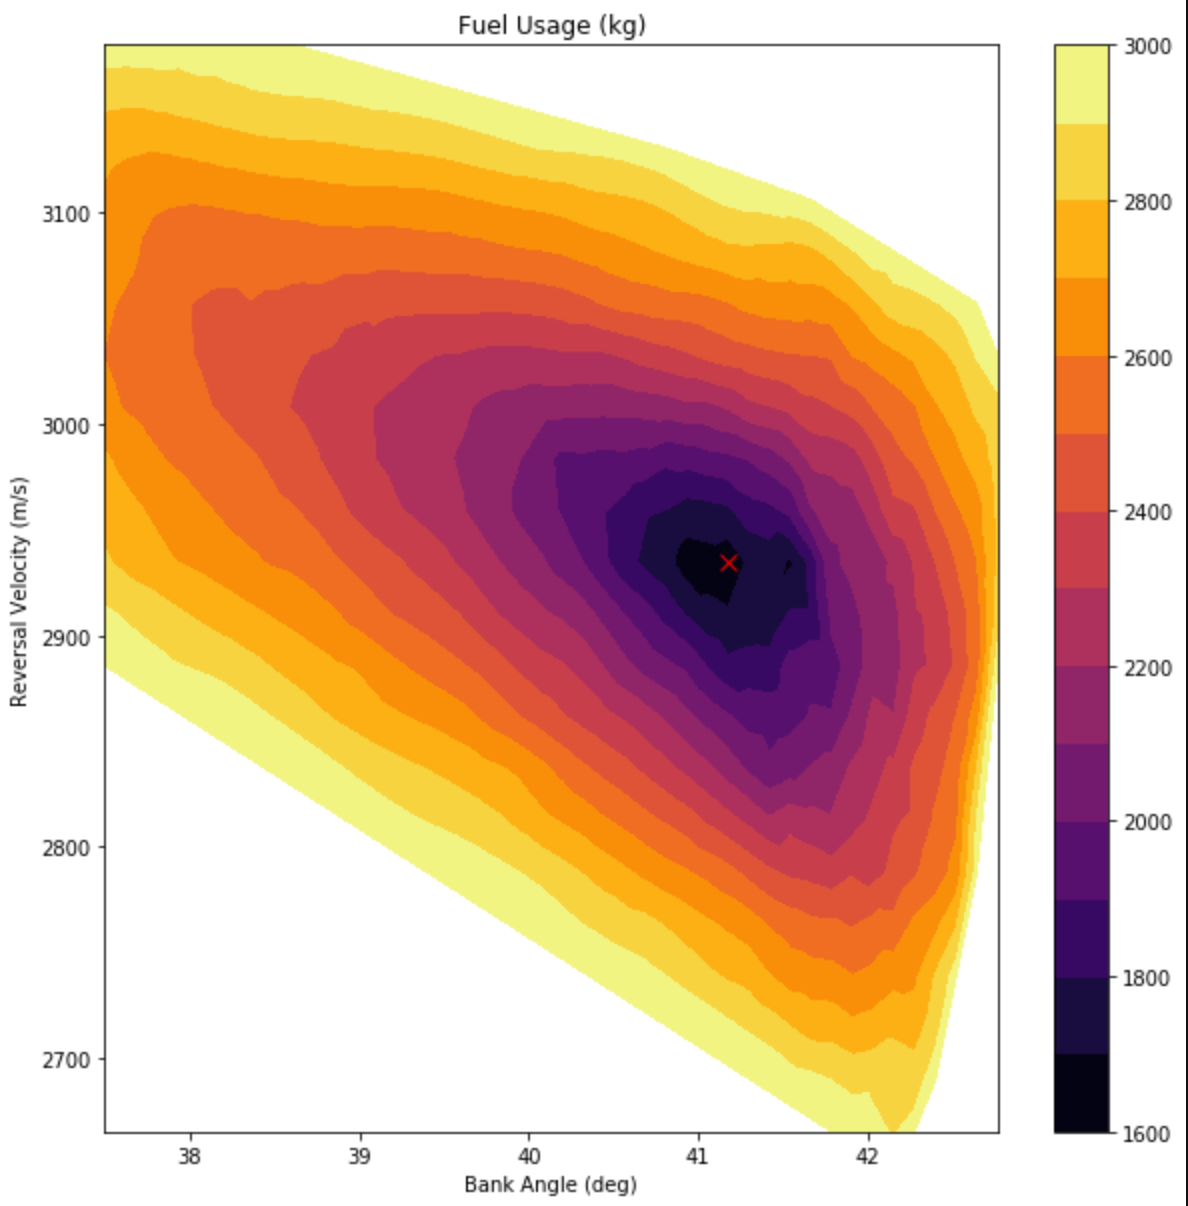
\includegraphics[width=0.9\textwidth]{Profile1_Objective} 
%		\caption{Contours of the objective function using a constant bank angle with one reversal, initial T/W = 16.}
%\end{figure}

%Contours of the optimal parameters corresponding to the solutions in Figure~\ref{fig_contour} are given in Figures~\ref{fig_bank} and \ref{fig_rev}. Immediately striking is the optimal bank angle's clear independence from azimuth errors; instead, it is dictated entirely by the flight path angle. 
%\begin{figure}[h!]
%	\centering
%	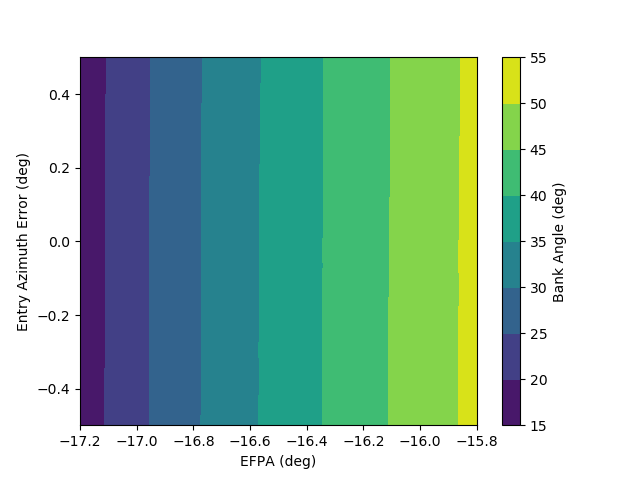
\includegraphics[width=1\textwidth]{optimal_bank} 
%	\caption{Optimal bank angle for different entry flight path angles and heading angles.}
%	\label{fig_bank}
%\end{figure}
%
%\begin{figure}[h!]
%	\centering
%	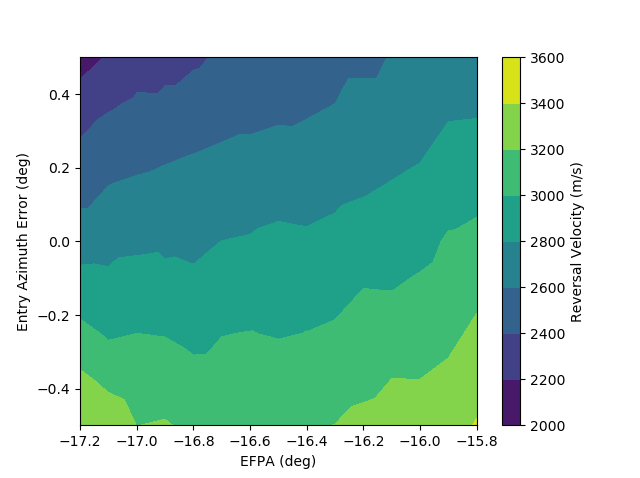
\includegraphics[width=1\textwidth]{optimal_reversal} 
%	\caption{Optimal reversal velocity for different entry flight path angles and heading angles.}
%	\label{fig_rev}
%\end{figure}
%
%
%\pagebreak
\section{Performance Assessment}
%TODO: Like the range error breakdown for different disturbances, show the propellant increases caused by different disturbances - i.e. sensitivity study ish?}
%TODO: Stability of predicted ignition conditions and propellant use over time. These variables form a path
%TODO: Seemingly very little variation in terminal entry state for different EFPA/AZI. But a standard feedback controller couldn't accomplish that 
\begin{table}[h!]
	\centering
	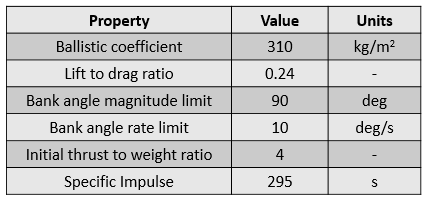
\includegraphics[width=0.6\textwidth]{ParamTable} 
	\caption{Model parameters used in all simulation results presented.}
	\label{table_model_params}
\end{table}
In order to characterize the behavior and performance of the entry guidance algorithm, simulations are conducted under various circumstances. In all examples, the vehicle under consideration has a nominal $L/D=0.24$, and a ballistic coefficient of $310\, \mathrm{kg/m^2}$, approximately double that of Mars 2020. The vehicle's propulsion model includes an initial $ T/W $ of 4 with a constant $ I_{sp} = 290$ s, and $T_{\min}=0.5T_{\max}$. These parameters are summarized in Table~\ref{table_model_params}.

The site targeted at the termination of the descent phase is 700 km downrange with $z_{\mathrm{target}}=\dot{z}_{\mathrm{target}}=0$. 
%The entry flight path angle in all examples is $ -15.75^\circ $. The vehicle's bank angle rate is limited to $10 ^{\circ}/s$. 
Performance is evaluated using the propellant mass fraction (PMF), the portion of the vehicle that is propellant, as the primary metric. The bounds used in the constraints Eq.~\ref{eq_constraints} are $z_{\min} = 3$ km, $[d_{\min},\,d_{\max}] = [0, 25]\,$ km, $v_{\max} = 700 $ m/s. The entry phase terminates at the ignition velocity last predicted by the entry guidance algorithm.

\subsection{Sensitivity Analysis}
The performance of the algorithm is first investigated in a series of one-dimensional sensitivities to parametric uncertainties, including lift and drag coefficients, and two forms of density uncertainty. For this section, the atmospheric density is modeled as 
\begin{align}
\rho = \rho_0\mathrm{e}^{-\frac{R-R_P}{h_s}}
\end{align}
where $\rho_0 = 0.0158 \,\mathrm{kg/m}^3$ is the density at the surface and $h_s = 9354.5$ m is the scale height. Uncertainty is modeled in each of these quantities. Variations in $\rho_0$ correspond to constant percentage shift at all altitudes, while variations in the scale height alter the density's gradient with respect to altitude, $\dfrac{\partial\rho}{\partial h} = -\dfrac{\rho}{h_s}$. The guidance algorithm is called at four fixed velocities, $5500, 4000, 2000,$ and $1000$ m/s.
%Entry state dispersions are also examined. 

Due to its reliance on predictions, the algorithm is susceptible to model uncertainty. Reference~\cite{predictor_corrector_analysis} examined the performance of predictive algorithms in the presence of such uncertainties and found, like Ref.~\cite{lu2014entry}, that model adaptation during flight is essential to good performance in the presence of such parametric uncertainty. In the simulations presented, trajectory predictions are made aerodynamic accelerations scaled ratios of current sensed accelerations to modeled accelerations, $L/L_{model}$ and $ D/D_{model} $. Because the first three perturbations result in constant ratios of $L/L_{model}$ and $ D/D_{model} $, the predictions will match the simulated environment, and the predicted propellant consumption and ignition state should not vary significantly with each call to the entry guidance algorithm. In contrast, the scale height uncertainty will result in aerodynamic ratios that vary with altitude, causing error in the predictions due to their inability to account for unknown future variations. Thus it is expected to see greater variation in the predicted propellant required as well as the predicted ignition state. This behavior is exhibited in Fig.~\ref{fig_parametric_updates}.
\begin{figure}[h!]
	\centering
	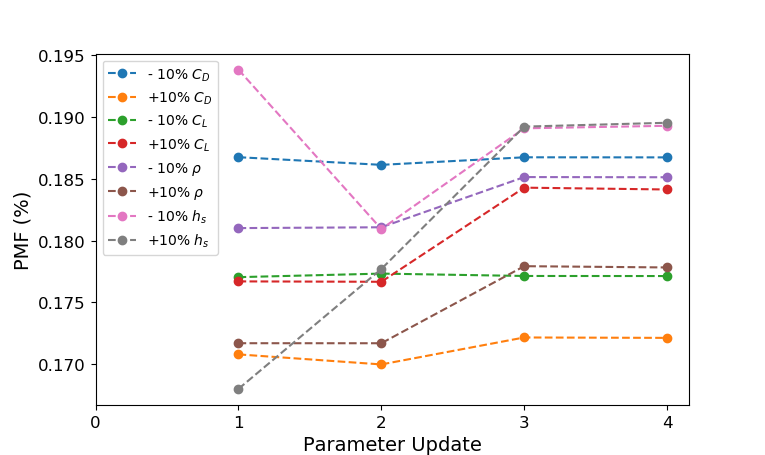
\includegraphics[width=0.7\textwidth]{ParameterUpdates} 
	\caption{The predicted PMF and associated ignition state may change each time the guidance algorithm is called. The solutions are less volatile when the discrepancy between the model predictions and the simulated environment is small. Larger variations in the solution due to variations in $h_s$ are expected since they result in unknown future density variations.}
	\label{fig_parametric_updates}
\end{figure}
\begin{table}[h!]
	\centering
	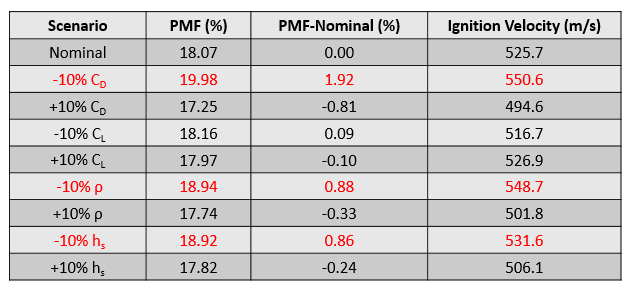
\includegraphics[width=0.75\textwidth]{ParametricSensitivityTable} 
	\caption{A summary of PMFs for a series of $\pm10\%$ uncertainties compared to a nominal scenario with no uncertainty. Scenarios with significant increases in PMF relative to the nominal scenario have been highlighted.}
	\label{table_parametric}
\end{table}
\begin{table}[h!]
	\centering
	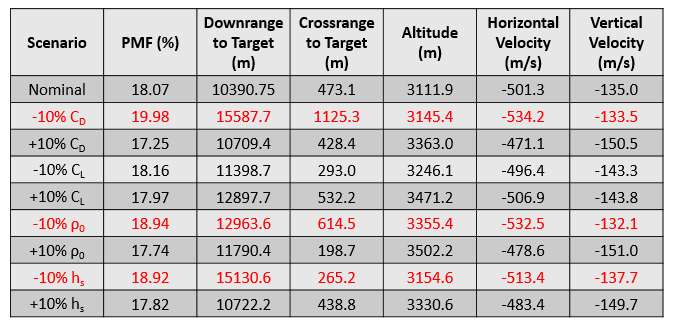
\includegraphics[width=0.8\textwidth]{ParametricSensitivityIgnitionTable} 
	\caption{A summary of the propellant-optimal ignition states for a series of $\pm10\%$ uncertainties. Optimal trajectories generally feature low crossrange, and altitudes close to the minimum altitude constraint.}
	\label{table_parametric_ignition}
\end{table}
\begin{figure}[h!]
	\centering
	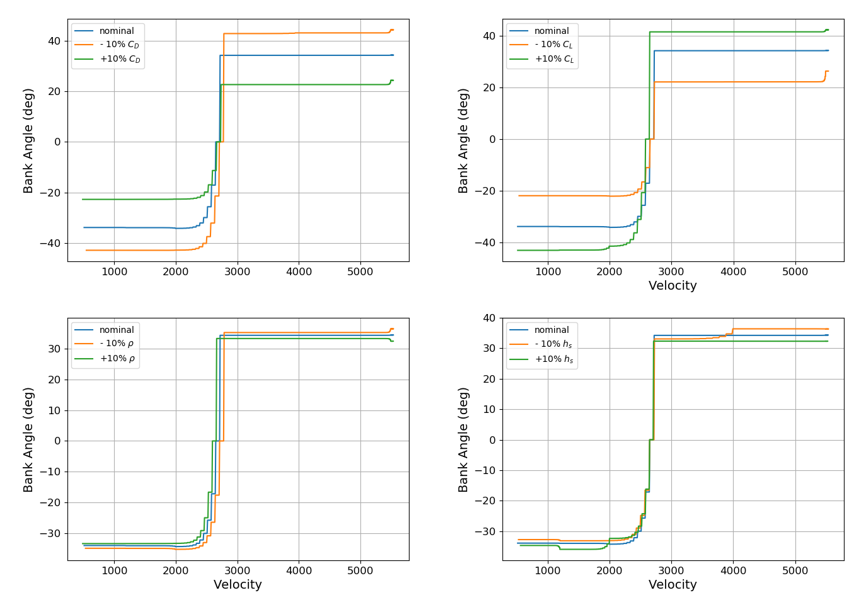
\includegraphics[width=0.9\textwidth]{SensitivityBankProfiles} 
	\caption{The bank angle profiles for a series of 1-D parametric sensitivities. Despite their similar effect on drag, the controller deals with $\pm C_D$ quite differently than $\pm \rho$.}
	\label{fig_parametric_bank}
\end{figure}

Figure~\ref{fig_parametric_bank} shows the resulting bank angle profiles. Due to their similar effect on the vehicle L/D ratio, the perturbations pairs  ($ +C_D $, $ -C_L $) and ($ -C_D $, $ +C_L $) result in essentially the same update to the bank angle magnitude. The lift dispersed cases essentially fly identical altitude-velocity profiles but have slightly different reversal velocities due to the impact of lift on lateral motion. 

Table~\ref{table_parametric} summarizes the PMF for each scenario and compares them to the nominal scenario, while Table~\ref{table_parametric_ignition} gives the corresponding propellant-optimal ignition states. Several trends are noticeable. The three scenarios with the highest PMF all involve lower than nominal drag acting on the vehicle, leading to higher ignition velocities and less favorable ignition states. Although the $-10\%\, \rho_0$ case features the same decrease in drag as $-10\%\,C_D$, it also preserves the $L/D$ ratio. Unlike the drag coefficient variations, the lift coefficient variations produced very little change in PMF.
There is a noticeable asymmetry present in each of the dispersions that affects drag: the minus variation, or ``low drag" scenario, requires a greater increase in PMF than is saved in the positive variation. Note that a constant $-10\%$ variation in drag (from any source) over the entire trajectory is a substantial perturbation that is challenging to overcome in the already thin atmosphere. Despite this, the additional PMF required relative to the nominal scenario is modest.

All of the trajectories feature lofting near the end of the entry phase (not shown), and the terminal altitude is almost always very close to the minimum altitude constraint. Since altitude decreases monotonically with velocity after lofting, this allows the vehicle to decelerate for as long as possible, reducing the velocity that must be nulled by SRP. Scenarios in which the optimal ignition occurs higher indicate some other constraint is active, such as overshooting the optimal downrange distance at which to ignite. Although there is no separate guidance logic for heading alignment, it is clear from the small crossrange values in Table~\ref{table_parametric_ignition} that by targeting the optimal point in $\mathcal{F}_M$, the vehicle heading is aligned prior to ignition. 

% For a fixed ground target, a wide range of entry flight path angles (EFPAs) and entry heading errors can be accommodated by the entry guidance algorithm. Figure~\ref{fig_sweep} is an example that demonstrates the propellant cost is approximately invariant with respect to entry azimuth errors and varies weakly with EFPA, about 200 kg of propellant over $1.4^\circ$ of variation in EFPA. The range of acceptable EFPAs is often set by considerations such as g-load limits, or aerothermal constraints, and these results indicate such constraints can be imposed at little-to-no cost to propellant. 
%
%It is expected that a guidance algorithm that provides range control during entry to the same downrange distance over such a range of EFPAs will fly very different entry trajectories with a much greater variance in the propellant cost to decelerate the vehicle while landing at the target. This is significant because vehicle designers will allocate propellant based on $3\sigma$ or high percentile estimates, and reducing both the mean and variance means potential for landing greater payload masses. A numerical assessment to quantify these effects...
%
%\begin{figure}[h!]
%	\centering
%	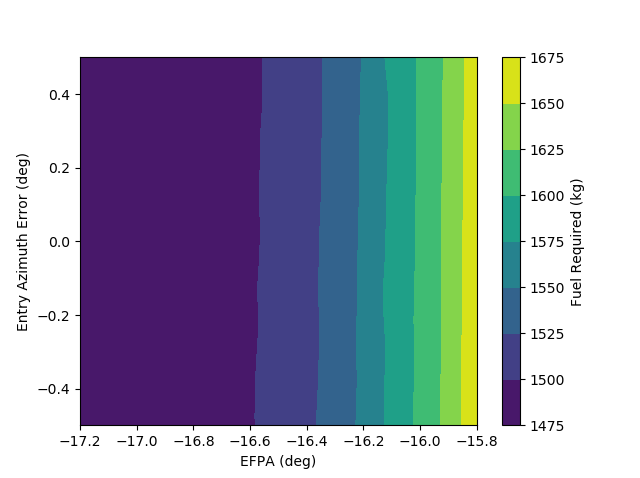
\includegraphics[width=1\textwidth]{optimal_fuel} 
%	\caption{Propellant required for different entry flight path angles and heading angles.}
%	\label{fig_sweep}
%\end{figure}

\subsection{Monte Carlo Simulation}
\begin{table}[h!]
	\centering
	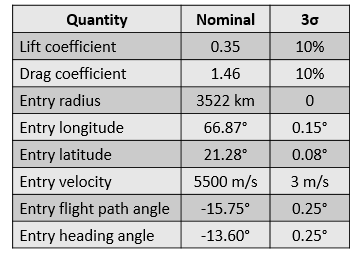
\includegraphics[width=0.4\textwidth]{DispersionTable} 
	\caption{The mean and $3\sigma$ values of the inputs used for the Monte Carlo simulation.}
	\label{table_input_dispersions}
\end{table}
\begin{figure}[h!]
	\centering
	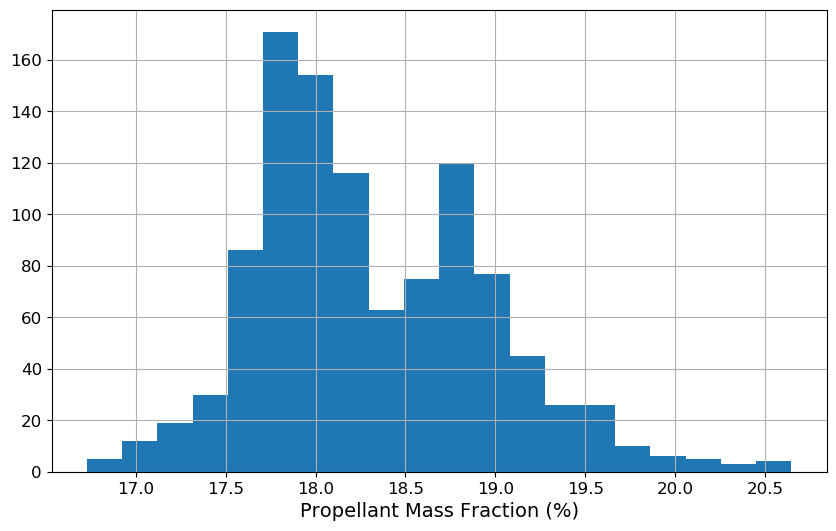
\includegraphics[width=0.6\textwidth]{ignition_pmf} 
	\caption{Propellant mass fraction for the Monte Carlo samples.}
	\label{fig_mc_pmf}
\end{figure}
\begin{figure}[h!]
	\centering
	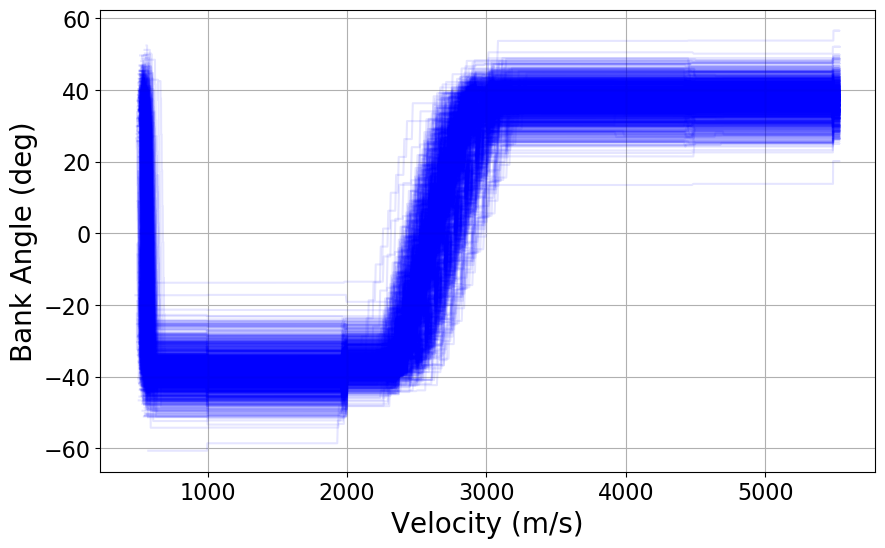
\includegraphics[width=0.6\textwidth]{bank_vel} 
	\caption{Bank angle profiles resulting from calls to the guidance algorithm at $ V=[5490, 4500, 3000, 2000, 1000] $ m/s.}
	\label{fig_mc_bank}
\end{figure}
\begin{figure}[h!]
	\centering
	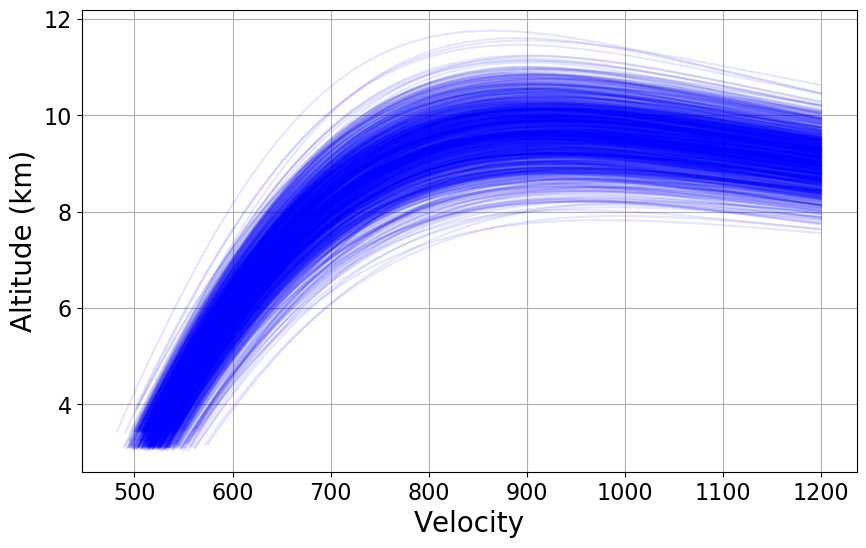
\includegraphics[width=0.6\textwidth]{alt_vel_zoomed} 
	\caption{All of the trajectories feature lofting as a means to further decelerate prior to ignition.}
	\label{fig_mc_alt_vel}
\end{figure}
\begin{figure}[h!]
	\centering
	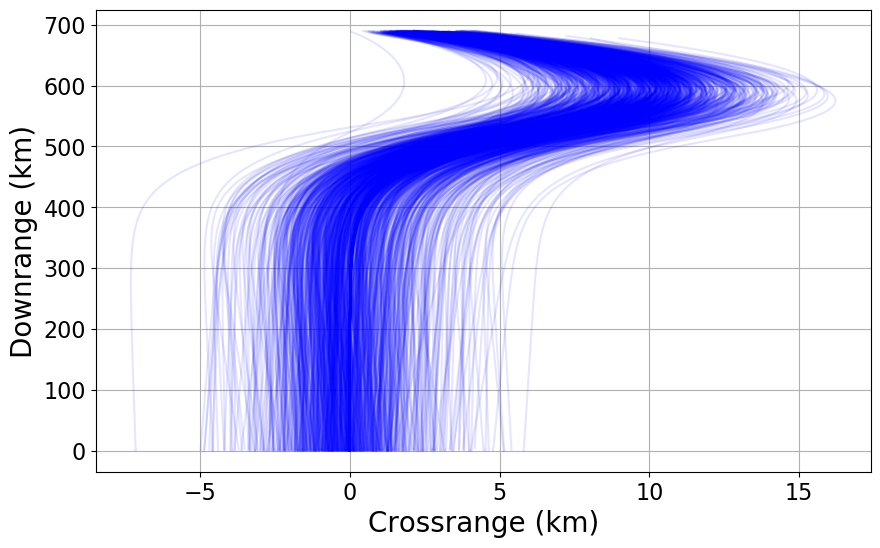
\includegraphics[width=0.6\textwidth]{dr_cr} 
	\caption{Downrange and crossrange flown from the entry state. Some trajectories fly significant crossranges due to the single planned bank reversal. Note that there are initial downrange errors in addition to than the initial crossrange errors, but due to the difference in scale they are not easily visible.}
	\label{fig_mc_entry_dr_cr}
\end{figure}
\begin{figure}[h!]
	\centering
	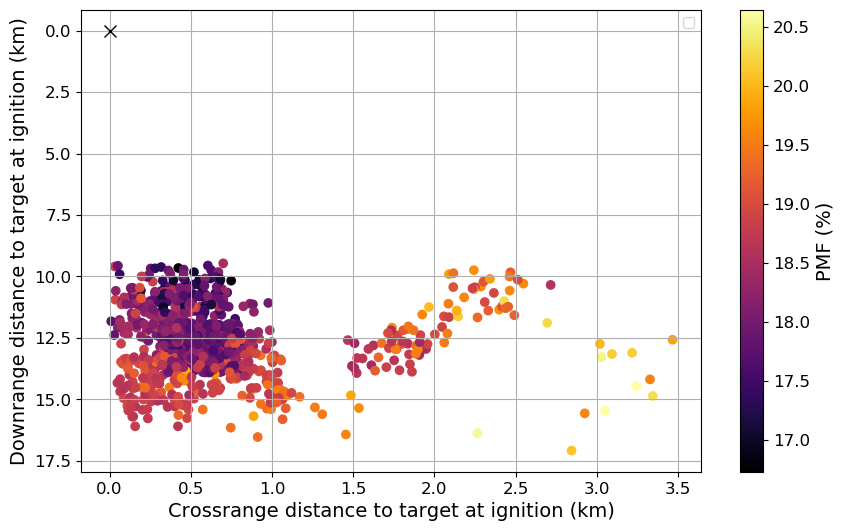
\includegraphics[width=0.7\textwidth]{ignition_dr_cr} 
	\caption{Downrange and crossrange to the target position. The crossrange is generally small, with 88\% under 1 km, indicating the vehicle heading is well-aligned at ignition.}
	\label{fig_mc_ignition_dr_cr}
\end{figure}
\begin{figure}[h!]
	\centering
	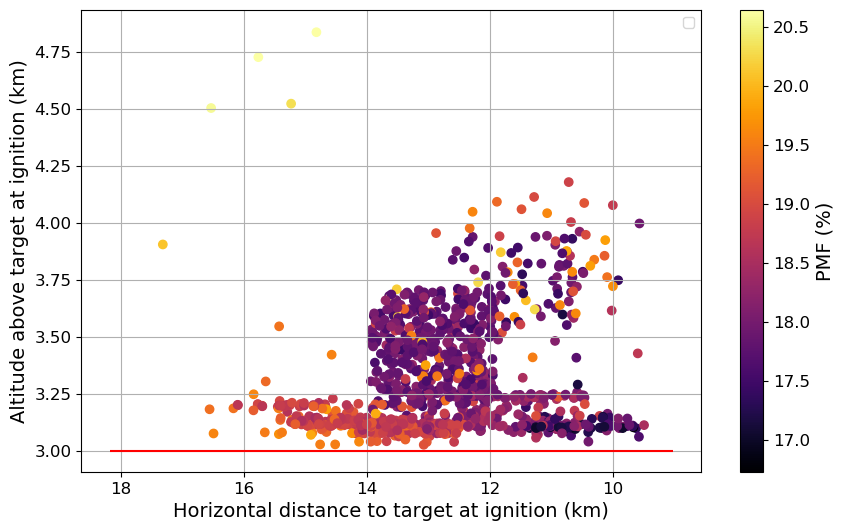
\includegraphics[width=0.7\textwidth]{ignition_alt_range} 
	\caption{The minimum altitude constraint, indicated in red, causes low energy scenarios to trigger at longer downrange distances and higher velocities, resulting in increased PMF.}
	\label{fig_mc_ignition_alt_vs_distance}
\end{figure}
\begin{figure}[h!]
	\centering
	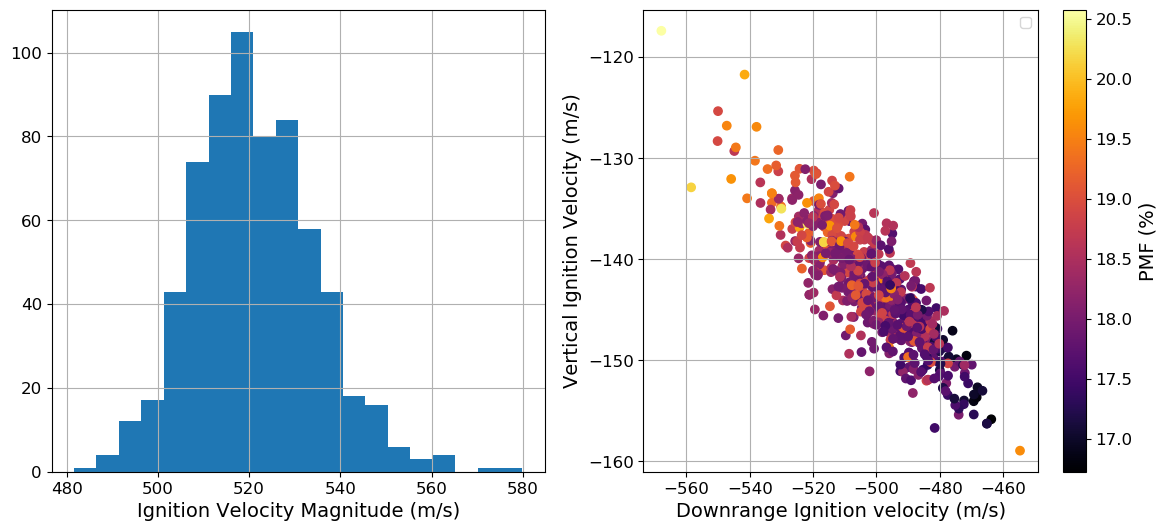
\includegraphics[width=0.9\textwidth]{ignition_vz_vx} 
	\caption{Ignition velocity magnitude (left) and components (right). Lower ignition velocities tend to occur at steeper flight path angles for the chosen parametrization. The correlation between velocity and PMF is evident, but the slowest ignition point (bottom right of the right plot) is nowhere near the lowest PMF value, demonstrating the importance of other state variables in determining the PMF required.}
	\label{fig_mc_ignition_vel}
\end{figure}
A Monte Carlo of 1000 samples is conducted with entry state delivery errors and aerodynamic dispersions, listed in Table~\ref{table_input_dispersions}, and a higher fidelity atmosphere model. The atmospheric density is modeled using MarsGRAM \cite{MarsGRAM2010User}, rather than the exponential model employed specifically for the sensitivity study. 
 
Figure~\ref{fig_mc_pmf} shows the distribution of PMFs and
Figs.~\ref{fig_mc_bank}-\ref{fig_mc_entry_dr_cr} display the entry trajectories. The median PMF is 18.2 \%, and the 99 percentile is 20.1\%. From Fig.~\ref{fig_mc_alt_vel} it is evident that all of the samples feature at least a mild lofting near the end of the entry phase. 
Figure~\ref{fig_mc_bank} depicts the bank angle profiles. The chosen parametrization of the bank profile, coupled with the nature of the disturbances modeled, means that unless significant perturbation of the vehicle heading occurs after the first reversal, there will be only one reversal in total. In instances where the prediction was inaccurate and the reversal was poorly timed as a result, a late second reversal is used to correct the vehicle heading. 

Figures~\ref{fig_mc_ignition_dr_cr}-\ref{fig_mc_ignition_vel} plot the ignition states at the ignition velocity determined by the last call to the entry guidance algorithm. For the vehicle under consideration, the optimal downrange to the target is generally between 10-15 km. Nearly all samples have a crossrange distance of less than 1 km at ignition, and the maximum crossrange samples trigger with around 3.5 km crossrange to the target. As seen in Fig.~\ref{fig_mc_ignition_vel}, ignition velocities occur over a range of nearly 100 m/s. PMF and velocity at ignition are naturally correlated, but the lowest velocity ignition (the point in the bottom right of the right plot) is near the upper end of the PMF range, which shows that other state variables may yet have a strong impact on the PMF required to land.

Figure~\ref{fig_mc_ignition_alt_vs_distance} shows that altitude at ignition is consistently low, within 1-2 km of the minimum altitude constraint. This is not surprising, as after the vehicle has passed the point of lofting, the lowest velocity along an entry trajectory will occur at the minimum altitude.
% Thus, low altitude ignitions are known to be optimal when the ignition flight path angles are shallow ($\le20^{\circ}$). 
%While this is the case for propellant-optimal powered descent solutions, it may not be true generally, i.e., for an alternative powered descent guidance. Nevertheless, 
The consistently low ignition altitudes suggest a guidance strategy that triggers ignition at a fixed altitude may perform nearly as well as searching for the optimal ignition state. Doing so would eliminate the need to find the optimum ignition point along a trajectory, removing the nested computation structure, and leaving only the optimization over the parameters of the bank angle profile. An additional benefit of such a strategy is a reduction of the propellant mapping interpolation to four dimensions, requiring far fewer solutions to represent the mapping with the same accuracy. Additionally, some of the suboptimality associated with an altitude trigger would be mitigated by the vehicle flying slightly differently knowing that the ignition altitude is different. 

Reference~\cite{PropellantOptimalAdaptiveTrigger} also noted that propellant-optimal ignitions generally occur near the last feasible entry state, but submits that propellant consumption alone is not a sufficient criterion for powered descent ignition because it does not account for operational margins. We suggest alternatively that by defining the minimum altitude constraint with operational margin in mind, the entry guidance algorithm may utilize an altitude trigger and focus exclusively on propellant consumption without issue. Another possible generalization is to trigger on a fixed glideslope angle, essentially allowing the final altitude to be lower if the vehicle is also nearer to the target.

\begin{figure}[h!]
	\centering
	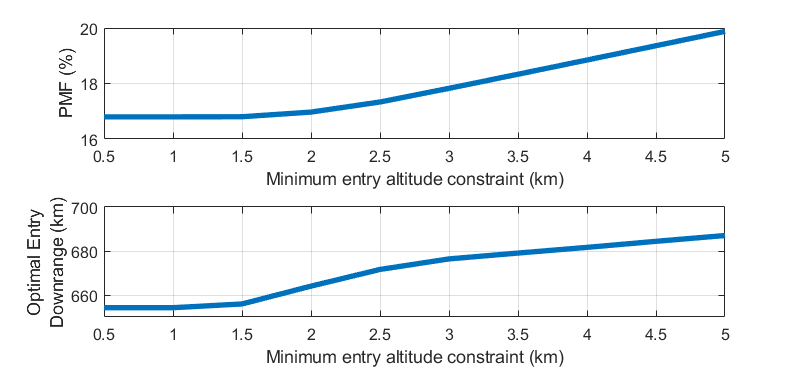
\includegraphics[width=0.9\textwidth]{min_alt_constraint} 
	\caption{The optimal placement of the target from the entry interface varies considerably with minimum entry altitude constraint has a strong impact on the geometry of the propellant optimal powered descent trajectories.}
	\label{fig_min_alt_constraint}
\end{figure} 
\begin{figure}[h!]
	\centering
	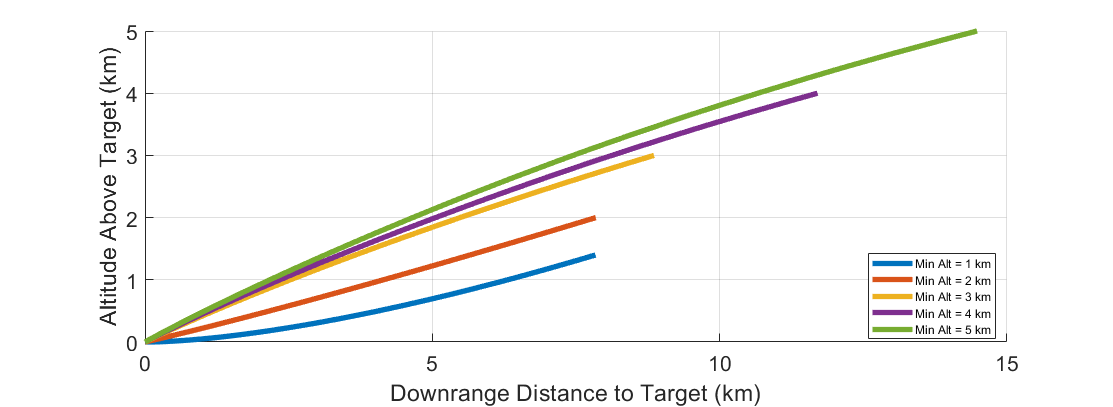
\includegraphics[width=0.9\textwidth]{SRP_vs_min_alt} 
	\caption{The minimum entry altitude constraint has a strong impact on the geometry of the propellant-optimal powered descent trajectories.}
	\label{fig_srp_traj}
\end{figure} 
 
 % %New stuff
The minimum altitude constraint also implications during mission design. Not only does it strongly affect the geometry of the powered descent phase, but it also affects the optimal entry trajectory length and the minimum propellant required.
 Figure~\ref{fig_min_alt_constraint} plots these quantities versus the value of the altitude constraint, while Fig.~\ref{fig_srp_traj} shows how the powered descent trajectories vary with the constraint. 
For the vehicle considered, and a constant bank angle magnitude during entry, the unconstrained optimal ignition altitude is about 1.5 km above the target. When the targeted downrange distance is free, the growth in PMF due to the constraint is modest, but the optimal entry downrange distance grows by nearly 40 km when imposing a 5 km constraint, and the propellant-optimal downrange distance from the target at ignition nearly doubles. 
 % %End New stuff
 
 
\section{Conclusion}
An entry guidance algorithm for chuteless, retropropulsion-based entry, descent, and landing was proposed. In particular, we addressed the problem of steering an entry vehicle to a propellant-optimal ignition condition. Feasible solutions to the powered descent problem are used to define the entry guidance target set. By computing and storing a mapping from ignition states in the target set to propellant required, the entry guidance algorithm maintains a predicted ignition state that varies over time as various perturbations alter the reachable set of the vehicle. The guidance algorithm updates the bank profile in order to track the propellant-optimal reachable state.

Although the role of entry guidance has always been to deliver the vehicle to favorable conditions for subsequent descent and landing phases, the use of the powered descent phase's guidance to define a target set, specifically for the purpose of reducing predicted powered descent propellant consumption, is novel. In parachute-based architectures, Mars entry guidance algorithms are generally judged on their ability to manage range errors while reaching the safe parachute deployment set. In contrast, in chuteless missions where pinpoint landing is achieved via powered descent, we posit that performance will instead be based on the required propellant to land the vehicle.

In the presented approach, the transition from the entry phase to powered descent is determined onboard during the optimization of the bank angle profile, but numerical results suggest that a possible simplification of the trigger is possible with little to no increase in propellant. Using a fixed altitude trigger would remove the need to optimize the ignition point along individual trajectories, and would allow a further reduction in size of the propellant map due to the decrease in dimensionality of the possible ignition states. The approach was demonstrated using a simple parametrization. Future work will consider alternatives, such as a profile designed specifically for achieving low velocity, which will likely yield lower propellant consumption. 
\bibliographystyle{AAS_publication}
\bibliography{bib}

\end{document}